
\hypertarget{Analyse-et-traitement-des-donnuxe9es}
\section{Les signaux}
\label{Les-signaux}}

Afin d'améliorer la lisibilité des chapitres suivant nous prendrons 3 signaux (le n°17000 et le n°20000 de la base labelisée ainsi que le n°571 de la base non labelisée) que nous observerons sous diverses formes puis sur lesquels nous effectuerons un certain nombre de traitements.

\hypertarget{Signaux-Bruts}{%}
\subsection{Signaux Bruts}
\label{Signaux-Bruts}}

Dans un premier temps on commence par observer les signaux sans traitements sous différentes formes.\n
D'abord de manière brute :

\begin{figure}[!h]
  \centering
  \begin{subfigure}[b]{0.3\textwidth}
    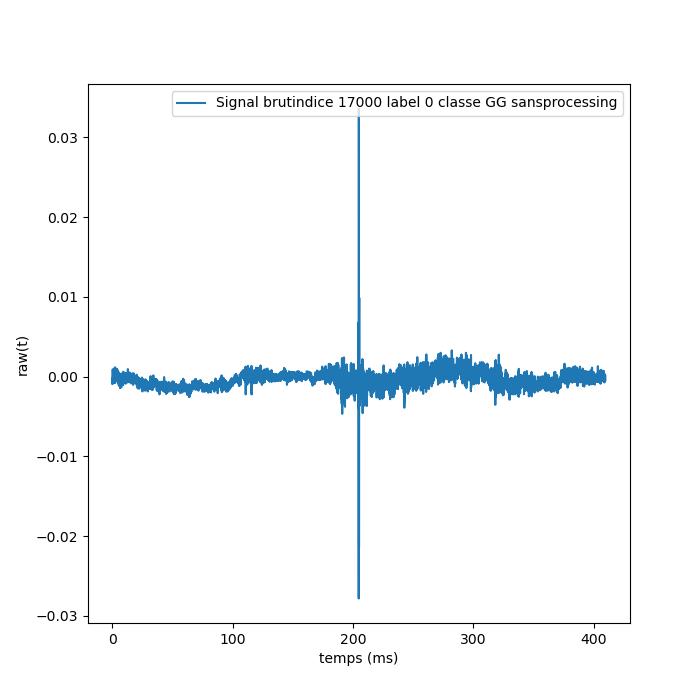
\includegraphics[width=\textwidth]{./images/indice17000Spectro1Dlabel0classeGGsansprocessingsanszoom.png}
  \end{subfigure}
  \begin{subfigure}[b]{0.3\textwidth}
    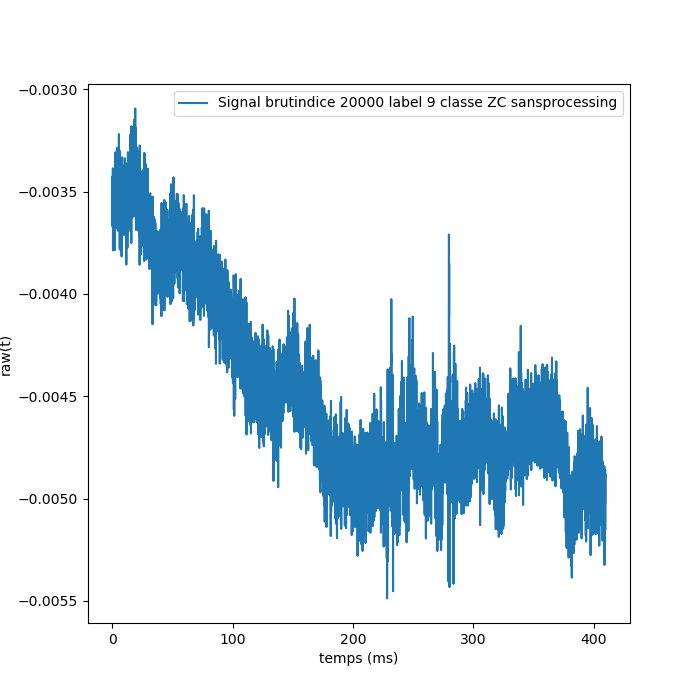
\includegraphics[width=\textwidth]{./images/indice20000Spectro1Dlabel9classeZCsansprocessingsanszoom.png}
    \caption{Signal 20000 brut}
  \end{subfigure}
  \begin{subfigure}[b]{0.3\textwidth}
    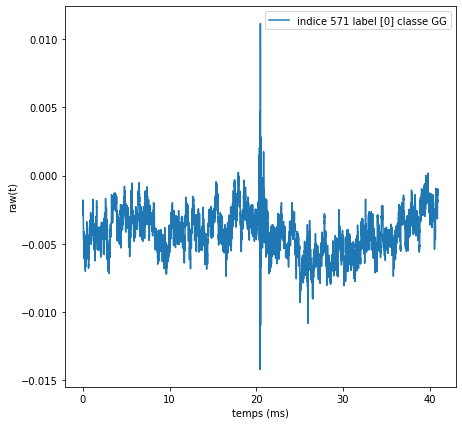
\includegraphics[width=\textwidth]{./images/indice571Spectro1Dlabel9classeZCsansprocessingsanszoom.png}
  \end{subfigure}
  \caption{Signaux 17000, 20000 et 571 bruts}
\end{figure}

On constate plusieurs choses tout d'abord il semble il y avoir une certaine disparité entre les signaux certains étant beaucoups plus bruités que d'autres. De plus contrairement a ce que l'on pouvais penser le clic n'est pas toujours facile a distinguer et celui ci n'est pas non plus toujours bien centré.
Cependant on peux tirer quelques observations :
-Le clic semble durer 5 millisecondes
-L'amplitude des clics semble variable
-Il arrive que le bruit soit parfois suffisament important par rapport au clic pour rendre sont identification complexe voir impossible
Pour afiner notre analyse il parait pertinent de commencer par zoomer sur ce clic.
Pour cela il vas donc faloir commencer par trouver un moyen d'isoler le clic.

\hypertarget{Le-zoom}{%}
\subsection{Le zoom}
\label{Le-zoom}}


\begin{figure}[!h]
  \centering
  \begin{subfigure}[b]{0.3\textwidth}
    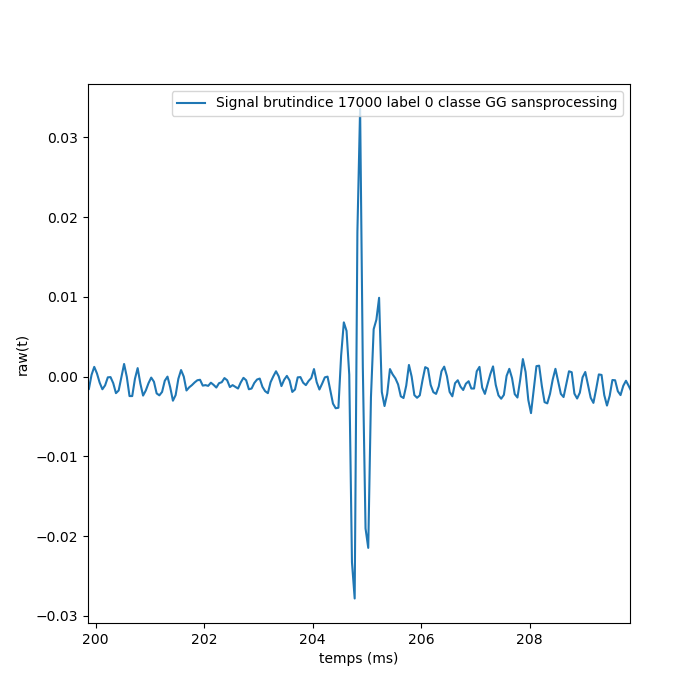
\includegraphics[width=\textwidth]{./images/indice17000Spectro1Dlabel0classeGGsansprocessingaveczoom.png}
  \end{subfigure}
  \begin{subfigure}[b]{0.3\textwidth}
    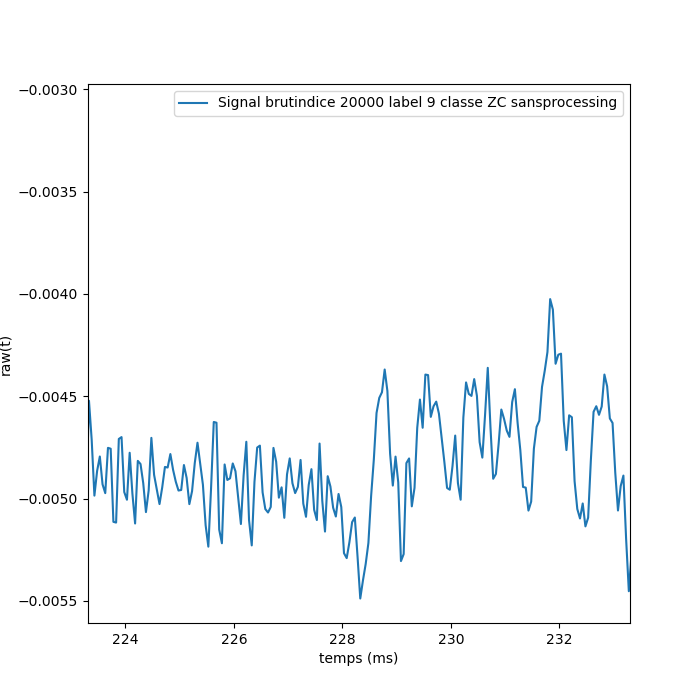
\includegraphics[width=\textwidth]{./images/indice20000Spectro1Dlabel9classeZCsansprocessingaveczoom.png}
  \caption{Signal 20000 zoom}
  \end{subfigure}
  \begin{subfigure}[b]{0.3\textwidth}
    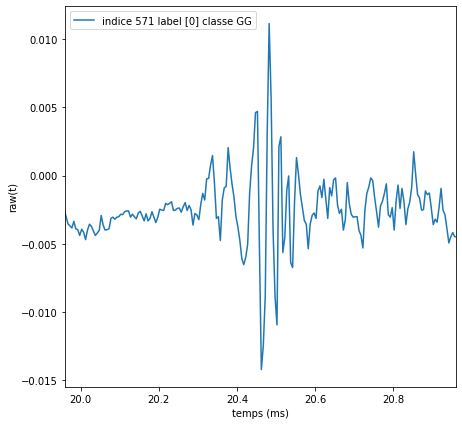
\includegraphics[width=\textwidth]{./images/indice571Spectro1Dlabel9classeZCsansprocessingaveczoom.png}
  \end{subfigure}
  \caption{Les signaux zoom}
\end{figure}

Pour zoomer sur le clic on commence par appliquer un filtre notament pour supprimer les bruits parasites(dont on parleras dans la partie traitement du signal) puis on identifie le maximum qui seras logiquement le milieux du clic puis on rajoute l'équivalent de la durée d'un clic avant et aprés ce maximum.

On constate plusieurs choses tout d'abord l'efficacité du zoom semble corélé a la qualité du signal de départ, de plus les "bons clics" semblent se situer aux alentours de 200 ms (ils sont donc bien centré) même si leur intensité semble très  variable pouvant aller jusqu'a un facteur 10 entre 2 clics. De plus sous cette forme nos observations semblent quand même limités. On vas donc commencer par les observer sous d'autres formes puis on chercheras a améliorer la qualité de nos signaux via diverses techniques. Etant donné la nature de nos données à savoir des enregistrements audios observer leurs spectrogrammes semble être le plus pertinent.

\hypertarget{Transformuxe9-de-Fourier}{%}
\subsection{Transformé de Fourier}
\label{Transformuxe9-de-Fourier}}
domaine temporel -> fréquenciel
Avant d'observer les spectrogrammes il convient de commencer par expliquer et observer les Transformés de Fourier de nos 3 signaux:
\begin{figure}[!h]
\centering
  \begin{subfigure}[b]{0.3\textwidth}
    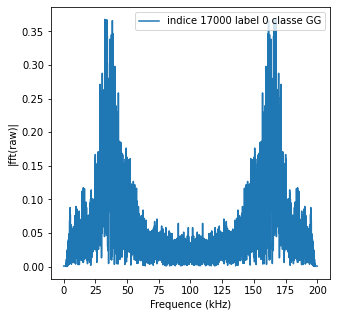
\includegraphics[width=\textwidth]{./images/17000fft.png}
  \end{subfigure}
  \begin{subfigure}[b]{0.3\textwidth}
    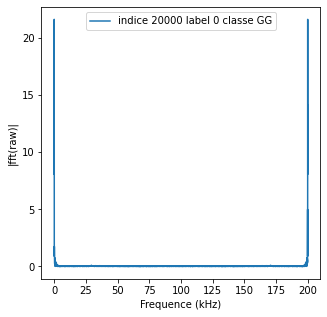
\includegraphics[width=\textwidth]{./images/20000fft.png}
  \end{subfigure}
  \begin{subfigure}[b]{0.3\textwidth}
    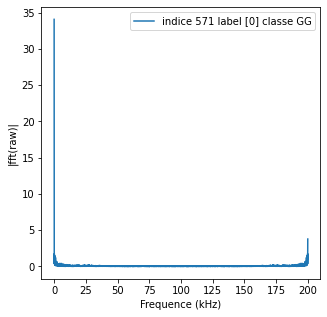
\includegraphics[width=\textwidth]{./images/571fft.png}
  \end{subfigure}
\caption{Transformé de Fourier des signaux 17000, 20000 et 571}
\end{figure}

\hypertarget{Spectrogrammes}{%}
\subsection{Spectrogrammes}
\label{Spectrogrammes}}

On commence tout d'abord par observer leurs Spectrogrammes en 2D:

\begin{figure}[!h]
  \centering
  \begin{subfigure}[b]{0.3\textwidth}
    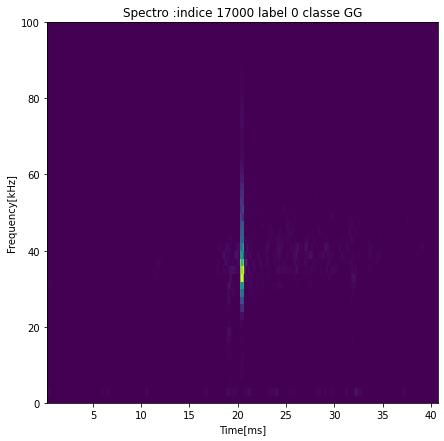
\includegraphics[width=\textwidth]{./images/indice17000Spectro2Dlabel0classeGGsansprocessingsanszoom.png}
  \end{subfigure}
  \begin{subfigure}[b]{0.3\textwidth}
    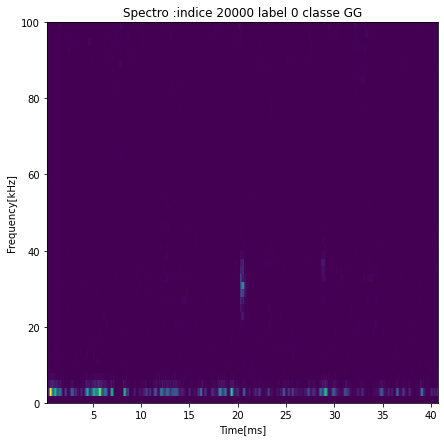
\includegraphics[width=\textwidth]{./images/indice20000Spectro2Dlabel9classeZCsansprocessingsanszoom.png}
  \end{subfigure}
  \begin{subfigure}[b]{0.3\textwidth}
    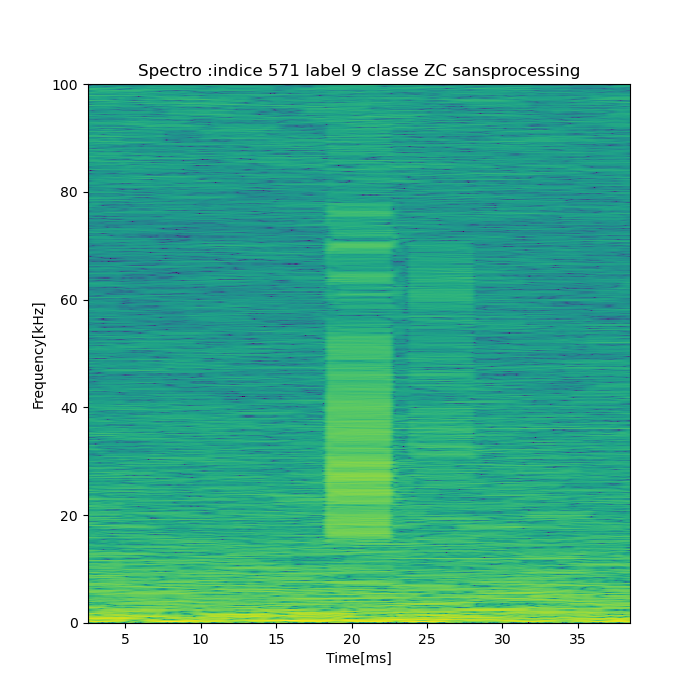
\includegraphics[width=\textwidth]{./images/indice571Spectro2Dlabel9classeZCsansprocessingsanszoom.png}
  \end{subfigure}
  \caption{Spectrogramme 2D des signaux}
\end{figure}

Puis les Spectrogrammes 3D:

\begin{figure}[!h]
\centering
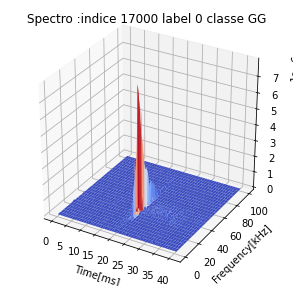
\includegraphics[width=4cm]{./images/indice17000Spectro3Dlabel0classeGGsansprocessingsanszoom.png}
\caption{Spectrogramme 3D du signal 17000}
\end{figure}
\begin{figure}[!h]
\centering
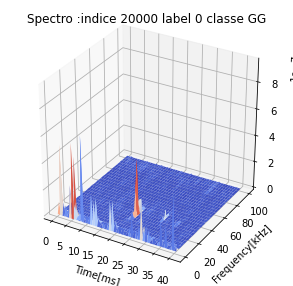
\includegraphics[width=4cm]{./images/indice20000Spectro3Dlabel9classeZCsansprocessingsanszoom.png}
\caption{Spectrogramme 3D du signal 20000}
\end{figure}

\begin{figure}[!h]
\centering
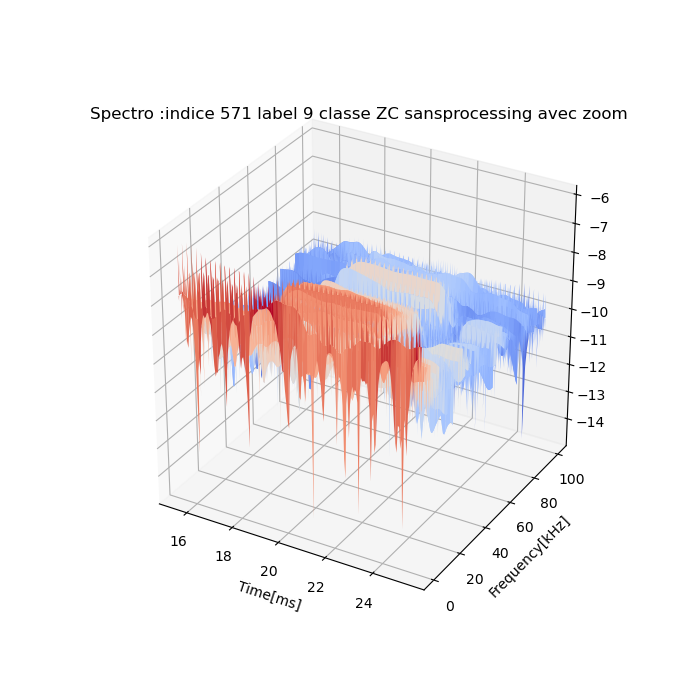
\includegraphics[width=4cm]{./images/indice571Spectro3Dlabel9classeZCsansprocessingaveczoom.png}
\caption{Spectrogramme 3D du signal 571}
\end{figure}

\hypertarget{Traitement-du-signal}
\subsection{Filtre passe haut}
\label{Filtre-passe-haut}}

\hypertarget{}
\section{Data augmentation}
\label{Data-augmentation}}

\hypertarget{}
\subsection{Rajout de bruit blanc}
\label{Rajout-de-bruit-blanc}}

\hypertarget{Simulation-de-distance}
\section{Les Pipelines}
\label{Les-Pipelines}}

%\hypertarget{}{%}
%\subsection{Présentation et interet des pipelines}
%\label{}}

\hypertarget{Les-PDF}
\chapter{Le travail à distance}\label{Le-travail-a-distance}}

\hypertarget{Organisation-du-travail-a-distance}{%}
\section{Organisation du travail à distance}\label{Organisation-du-travail-a-distance}}


Comme vous le savez certainement durant cette année 2020 nous avons été touchés par la crise du coronavirus qui nous a conduit a être confinés nous forçant a travailler uniquement a distance.

Ces circonstances très particuliéres ont grandement affecté notre travail particulérement au début ou nous avons du régler de nombreux problémes techniques et organisationels. Cependant en nous forçant a nous adapter a ces nouvelles conditions, cette crise nous a permis de grandement augmenter nos competances en "télétravail".

Ainsi malgrés des débuts léthargiques nous avons mis en place une "routine de travail" qui était la suivante :
-Des visio-conférences quotidiennes nous permettant d'organiser et de synchroniser notre travail
-Un groupe whatsap dédié a mon stage afin de communiquer le plus efficacement possible
-Un Github privé dédié afin de partager l'ensemble du projet
-Un partage régulier de google collab via google drive


\hypertarget{Outils-utilisuxe9s}
\subsection{Présentation de GitHub}
\label{Pruxe9sentation-de-GitHub}}

\begin{figure}[h]
  \begin{center}
  
\includegraphics[width=5cm]{./images/github.jpg}
  \end{center}
\end{figure}

Nous pouvons définir GitHub comme une plateforme de développement de projet in formatique en groupe. Elle s'implifie grandement le développement de projets. Elle permet de versioner ses programme et d'y apporter des modification en temps réel à plusieurs.

\hypertarget{Pourquoi-Github}{%}
\subsubsection{Pourquoi Github}
\label{Pourquoi-Github}}
Car celà permet une certaine synergie avec nos autres outils que nou verrons plus tard. Cette plateforme permet une facilité de développement de par sa fonctionnalité de versionnage de notre code à chaque changement ce qui permet une mise à jour dynamique ainsi que une relative facilitée a retourner à un état entérieur de notre programme ce qui permet une faciliter de débogage.Nous pouvons d'ailleur dire que ce rappport est entreposer sur Github et qu'il peut être récupérer facilement.Cette plateforme est aussi très connu dans le monde de la programmation ce qui sera utile pour notre future professionnel.

\hypertarget{Pruxe9sentation-de-Google-Colab}{%}
\subsection{Présentation de Google Colab}
\label{Pruxe9sentation-de-Google-Colab}}

\begin{figure}[h]
\begin{center}

\includegraphics[width=5cm]{./images/Colab_logo.png}
\end{center}
\end{figure}

Colab peut-être défini comme étant une plateforme d'éxécution pour notre code
il permet du fait que ce soit la puissance de calcul d'ordinateur géré par Google une vitesse d'exécution ainsi qu'une vitesse de téléchargement de base de données supérieur à celle qui nous est disponible en local.

\hypertarget{Pourquoi-Colab}{%}
\subsubsection{Pourquoi Colab}
\label{Pourquoi-Colab}}
En premier lieu pour la faciliter d'exéccution du code car ce n'est pas en local ce qui permet une exécution quasi immédiate du code sans aucune installation.Il est aussi facile de mettre sur github du code produit avec colab car c'est deux plateforme sont liées. Il permet de par l'utilisation du format Jupyter de mélanger code et texte (peu aussi comporter des images) dans notre notebook.

Voilà un exmple d'exécution avec colab:

\begin{figure}[h]
\begin{center}
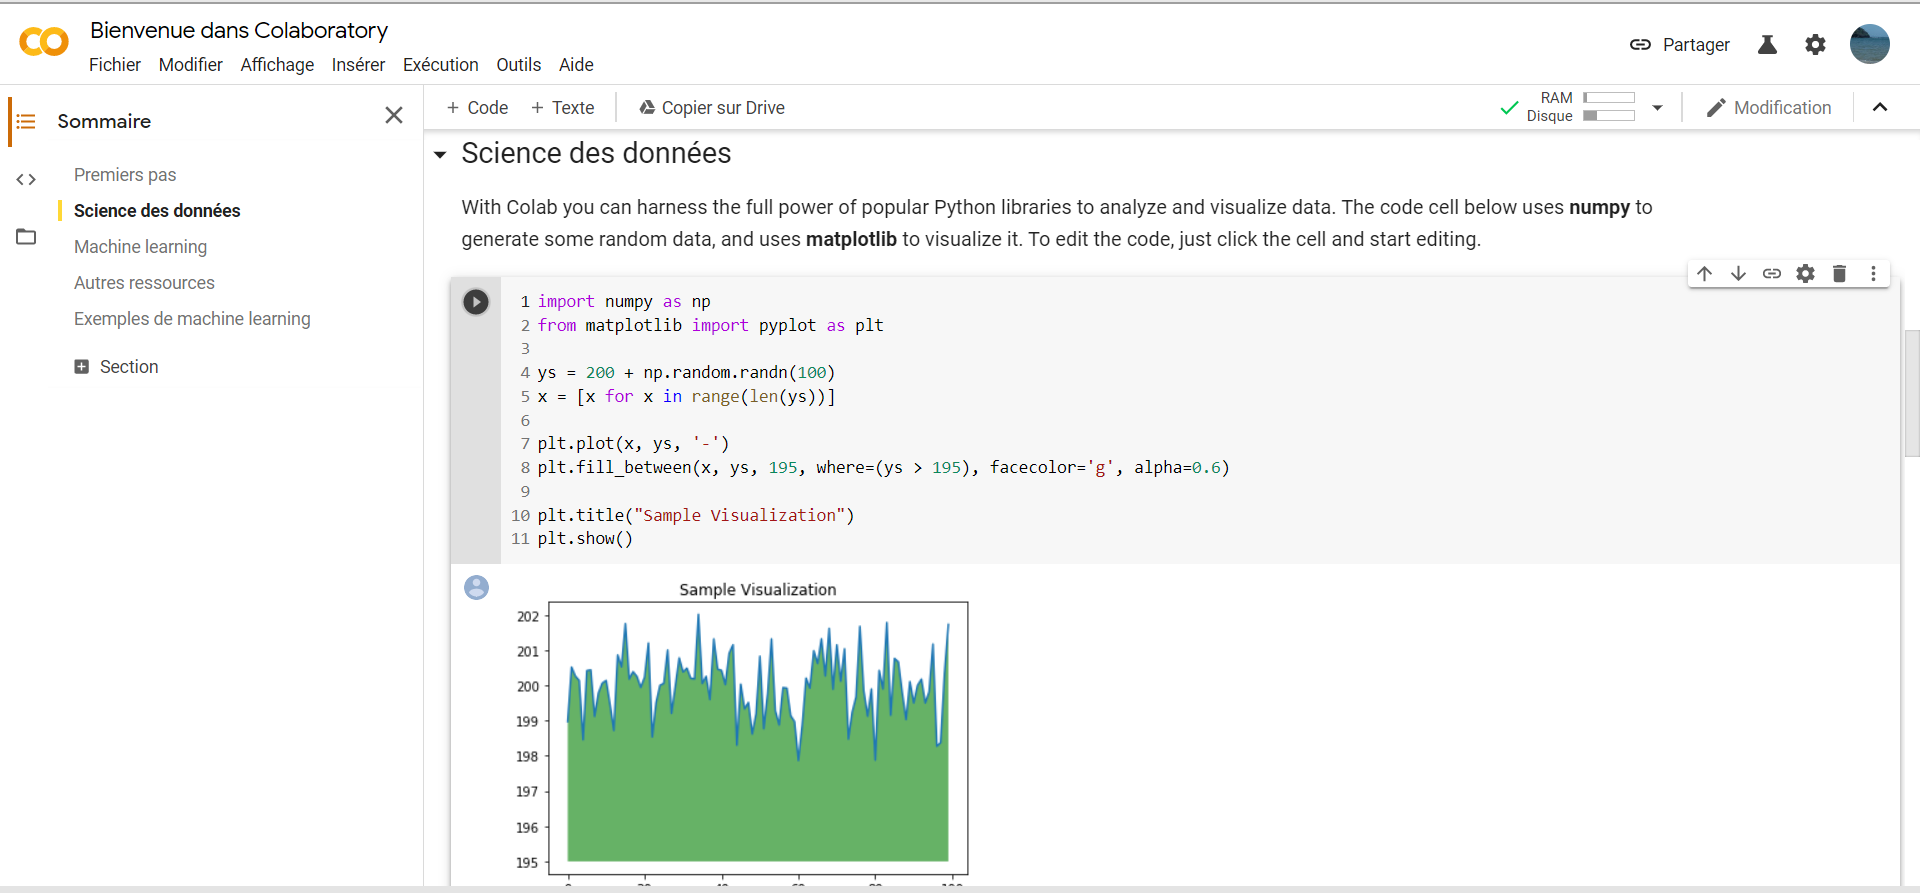
\includegraphics[width=15cm]{./images/Cap_colab.PNG}
\caption{Nous avons ici un exemple de code exécuté avec colab.}
\end{center}
\end{figure}


\hypertarget{Pruxe9sentation-de-LaTex}{%}
\subsection{Présentation de LaTex}
\label{Pruxe9sentation-de-LaTex}}

\begin{figure}[h]
  \begin{center}

\includegraphics[width=5cm]{./images/Latex.png}
\end{center}
\end{figure}

Nous pouvons dire que LaTex est un langage de traitement de texte tel que le markdown qui permet de mettre en forme notre texte de manière \"scientifique\" cela veut dire que. LaTex permet une faciliter d'écriture des équations et de toutes les écriture mathématiques.Permet de par ses nombreux package une quasi-infinité de possibilitées.
